\begin{itemize}
    \item Question type distribution. 
    We sample 200 questions from the training set and partition them into various categories shown in Table \tabref{main_examples}.\\
    1.) bidaf answers like "10-20" and true answer: 10
    2.) count numbe of occurences 
%     We curate most frequently occurring top 200 bi-gram and tri-gram patterns and partition them into different categories based on domain knowledge. For example, the patterns with words ``longest", ``shortest"", and farthest etc. would require sorting.
%   This heuristic-based approximate question distribution is shown in \figref{answer_distrib}
    \item types of reasoning needed to answer questions \tabref{interesting_example}
    \item distribution of answer types - span, number, digit
    \item What's \emph{not} in the data: common sense inference, except for lexical relationships (e.g., grandfather $==$ mother's father).  Some questions require knowledge of scoring in sports; there are enough examples of these that the model at least has a chance of learning this from the data.
\end{itemize}

% \begin{figure}
%     \centering
%     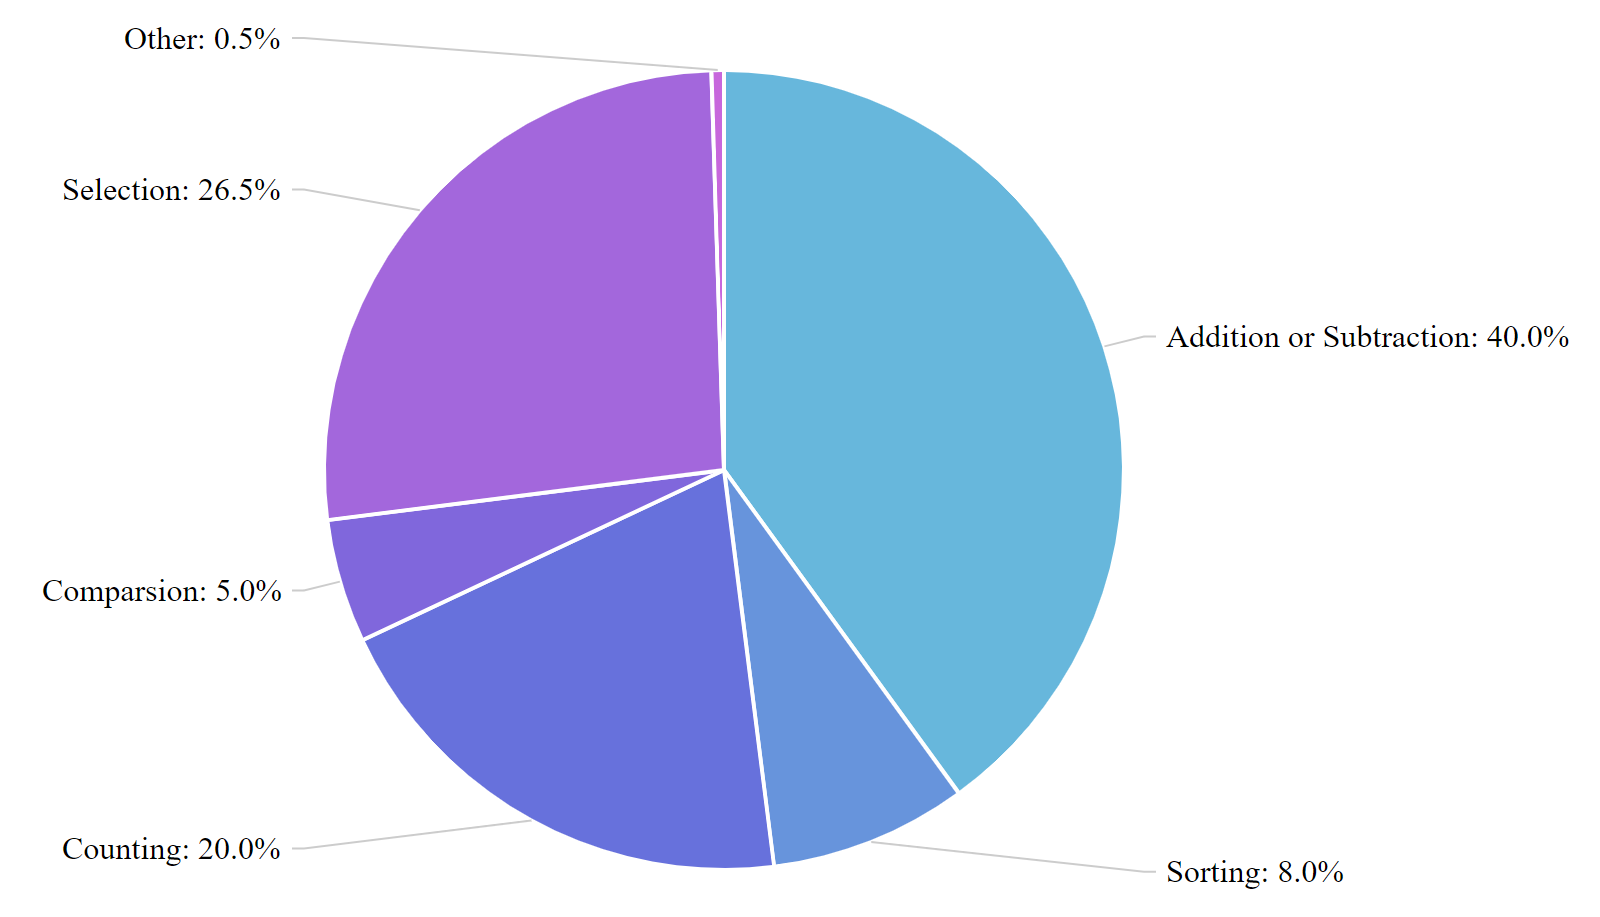
\includegraphics[width=0.5\textwidth]{images/answer_distrib}
%     \caption{Distribution of categories of questions}
%     \label{fig:answer_distrib}
% \end{figure}
% \gabi{Consider removing this figure 
% and putting numbers in Table 1}
% \sameer{Agreed!}